\documentclass{article}
\usepackage{physics}
\usepackage{graphicx}
\usepackage{caption}
\usepackage{amsmath}
\usepackage{bm}
\usepackage{framed}
\usepackage{authblk}
\usepackage{empheq}
\usepackage{amsfonts}
\usepackage{esint}
\usepackage[makeroom]{cancel}
\usepackage{dsfont}
\usepackage{centernot}
\usepackage{mathtools}
\usepackage{subcaption}
\usepackage{bigints}
\usepackage{amsthm}
\theoremstyle{definition}
\newtheorem{lemma}{Lemma}
\newtheorem{defn}{Definition}[section]
\newtheorem{prop}{Proposition}[section]
\newtheorem{rmk}{Remark}[section]
\newtheorem{thm}{Theorem}[section]
\newtheorem{exmp}{Example}[section]
\newtheorem{prob}{Problem}[section]
\newtheorem{sln}{Solution}[section]
\newtheorem*{prob*}{Problem}
\newtheorem{exer}{Exercise}[section]
\newtheorem*{exer*}{Exercise}
\newtheorem*{sln*}{Solution}
\usepackage{empheq}
\usepackage{tensor}
\usepackage{xcolor}
%\definecolor{colby}{rgb}{0.0, 0.0, 0.5}
\definecolor{MIT}{RGB}{163, 31, 52}
\usepackage[pdftex]{hyperref}
%\hypersetup{colorlinks,urlcolor=colby}
\hypersetup{colorlinks,linkcolor={MIT},citecolor={MIT},urlcolor={MIT}}  
\usepackage[left=1in,right=1in,top=1in,bottom=1in]{geometry}

\usepackage{newpxtext,newpxmath}
\newcommand*\widefbox[1]{\fbox{\hspace{2em}#1\hspace{2em}}}

\newcommand{\p}{\partial}
\newcommand{\R}{\mathbb{R}}
\newcommand{\C}{\mathbb{C}}
\newcommand{\lag}{\mathcal{L}}
\newcommand{\nn}{\nonumber}
\newcommand{\ham}{\mathcal{H}}
\newcommand{\M}{\mathcal{M}}
\newcommand{\I}{\mathcal{I}}
\newcommand{\K}{\mathcal{K}}
\newcommand{\F}{\mathcal{F}}
\newcommand{\w}{\omega}
\newcommand{\lam}{\lambda}
\newcommand{\al}{\alpha}
\newcommand{\be}{\beta}
\newcommand{\x}{\xi}

\newcommand{\G}{\mathcal{G}}

\newcommand{\f}[2]{\frac{#1}{#2}}

\newcommand{\ift}{\infty}

\newcommand{\lp}{\left(}
\newcommand{\rp}{\right)}

\newcommand{\lb}{\left[}
\newcommand{\rb}{\right]}

\newcommand{\lc}{\left\{}
\newcommand{\rc}{\right\}}


\newcommand{\V}{\mathbf{V}}
\newcommand{\U}{\mathcal{U}}
\newcommand{\Id}{\mathcal{I}}
\newcommand{\D}{\mathcal{D}}
\newcommand{\Z}{\mathcal{Z}}

%\setcounter{chapter}{-1}


\usepackage{enumitem}



\usepackage{listings}
\captionsetup[lstlisting]{margin=0cm,format=hang,font=small,format=plain,labelfont={bf,up},textfont={it}}
\renewcommand*{\lstlistingname}{Code \textcolor{violet}{\textsl{Mathematica}}}
\definecolor{gris245}{RGB}{245,245,245}
\definecolor{olive}{RGB}{50,140,50}
\definecolor{brun}{RGB}{175,100,80}

%\hypersetup{colorlinks,urlcolor=colby}
\lstset{
	tabsize=4,
	frame=single,
	language=mathematica,
	basicstyle=\scriptsize\ttfamily,
	keywordstyle=\color{black},
	backgroundcolor=\color{gris245},
	commentstyle=\color{gray},
	showstringspaces=false,
	emph={
		r1,
		r2,
		epsilon,epsilon_,
		Newton,Newton_
	},emphstyle={\color{olive}},
	emph={[2]
		L,
		CouleurCourbe,
		PotentielEffectif,
		IdCourbe,
		Courbe
	},emphstyle={[2]\color{blue}},
	emph={[3]r,r_,n,n_},emphstyle={[3]\color{magenta}}
}






\begin{document}
\begin{framed}
\noindent Name: \textbf{Huan Q. Bui}\\
Monday, Oct 17, 2022\\
BEC1 mask fabrication proposal \\
PI: Prof. Martin Zwierlein
\end{framed}


\noindent \textbf{1. Purpose}\\



\noindent \textbf{2. Procedure}

\begin{enumerate}[label=(\alph*)]

\item Acquire Thorlabs' \href{https://www.thorlabs.com/thorproduct.cfm?partnumber=WL11050-C7}{WL11050-C7} glass window. Material N-BK7. Diameter: 1 inch. The glass window is AR-coated, suitable for 400-700 nm. The mask will be created on this glass window blank. \vspace{-11pt}
\begin{figure}[!htb]
\centering
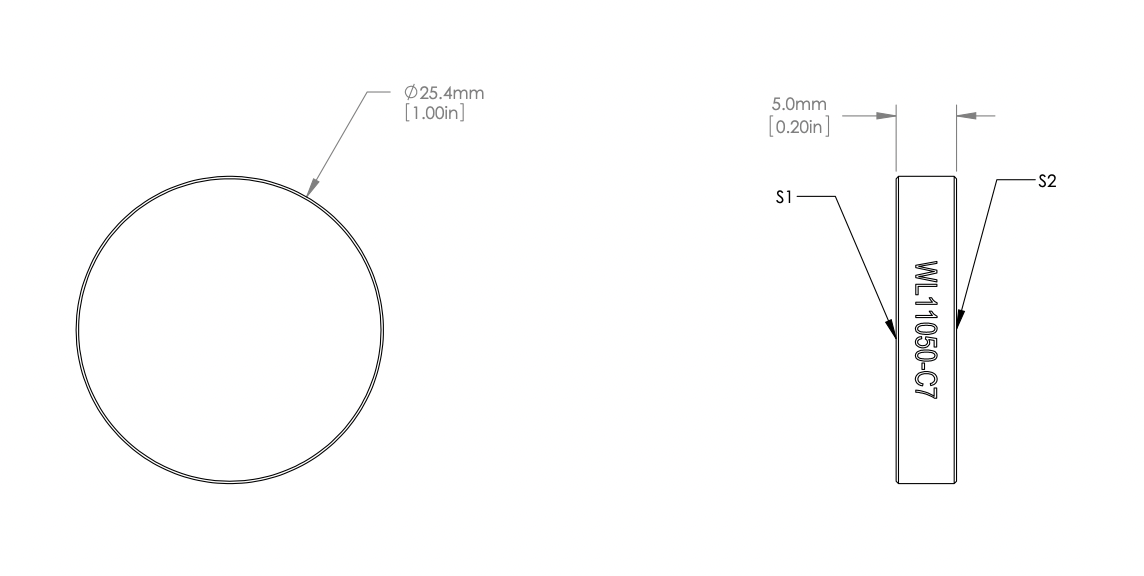
\includegraphics[scale=0.6]{thorlabs_window.png}
\end{figure}
\vspace{-20pt}

Other specifications:
\begin{itemize}
\item Surface flatness: $\leq \lambda/10$ at 633 nm

\item Surface quality: 10-5 scratch-dig

\item Thickness tolerance: $\pm 0.3$ mm 

\item Parallelism: $\leq 5$ arcsec
\end{itemize}


\item Clean the N-BK7 window with acetone, followed by methanol, followed by IPA. Blow dry with N$_2$.

\item Spin AZ3312 (positive) photoresist to approximately 400 nm thickness.

\item Expose pattern with the MLA150 machine.

\item Develop substrate. Time and temperature: to be determined.

\item Deposit a layer of silver (Ag) with thickness of 150 nm.

\item Silver liftoff: remove the photoresist and the silver that was deposited on the resist in the Microposit Remover 1165 overnight. 

\item Solvent clean using acetone, followed by methanol, followed by IPA. Blow dry with N$_2$.

\item Deposit a 20 nm-thick layer of SiO$_2$ on the entire substrate using CVD.

\end{enumerate}


\end{document}











